\section{Mechanical test setup}\label{sec:Mechanical_testsetup.tex}
The mechanical test setup available at Aalborg University can be seen on \figref{fig:Mec_abcd}. It includes four of the motors described in \secref{Maxon_Motor} attached to the four rotational plates seen on \figref{fig:Mec_a} and \figref{fig:Mec_b}. These plates connect the motors and the EndoWrist, such that the EndoWrist can be manipulated. See \figref{fig:Mec_c} and \figref{fig:Mec_d} for the attachment of the EndoWrist to the EndoWrist holder.  

\begin{figure}[H]
	\centering
	\begin{minipage}[t]{0.9\textwidth}
	\begin{subfigure}{0.45\textwidth}
		\vspace{-10pt}
		\centering
		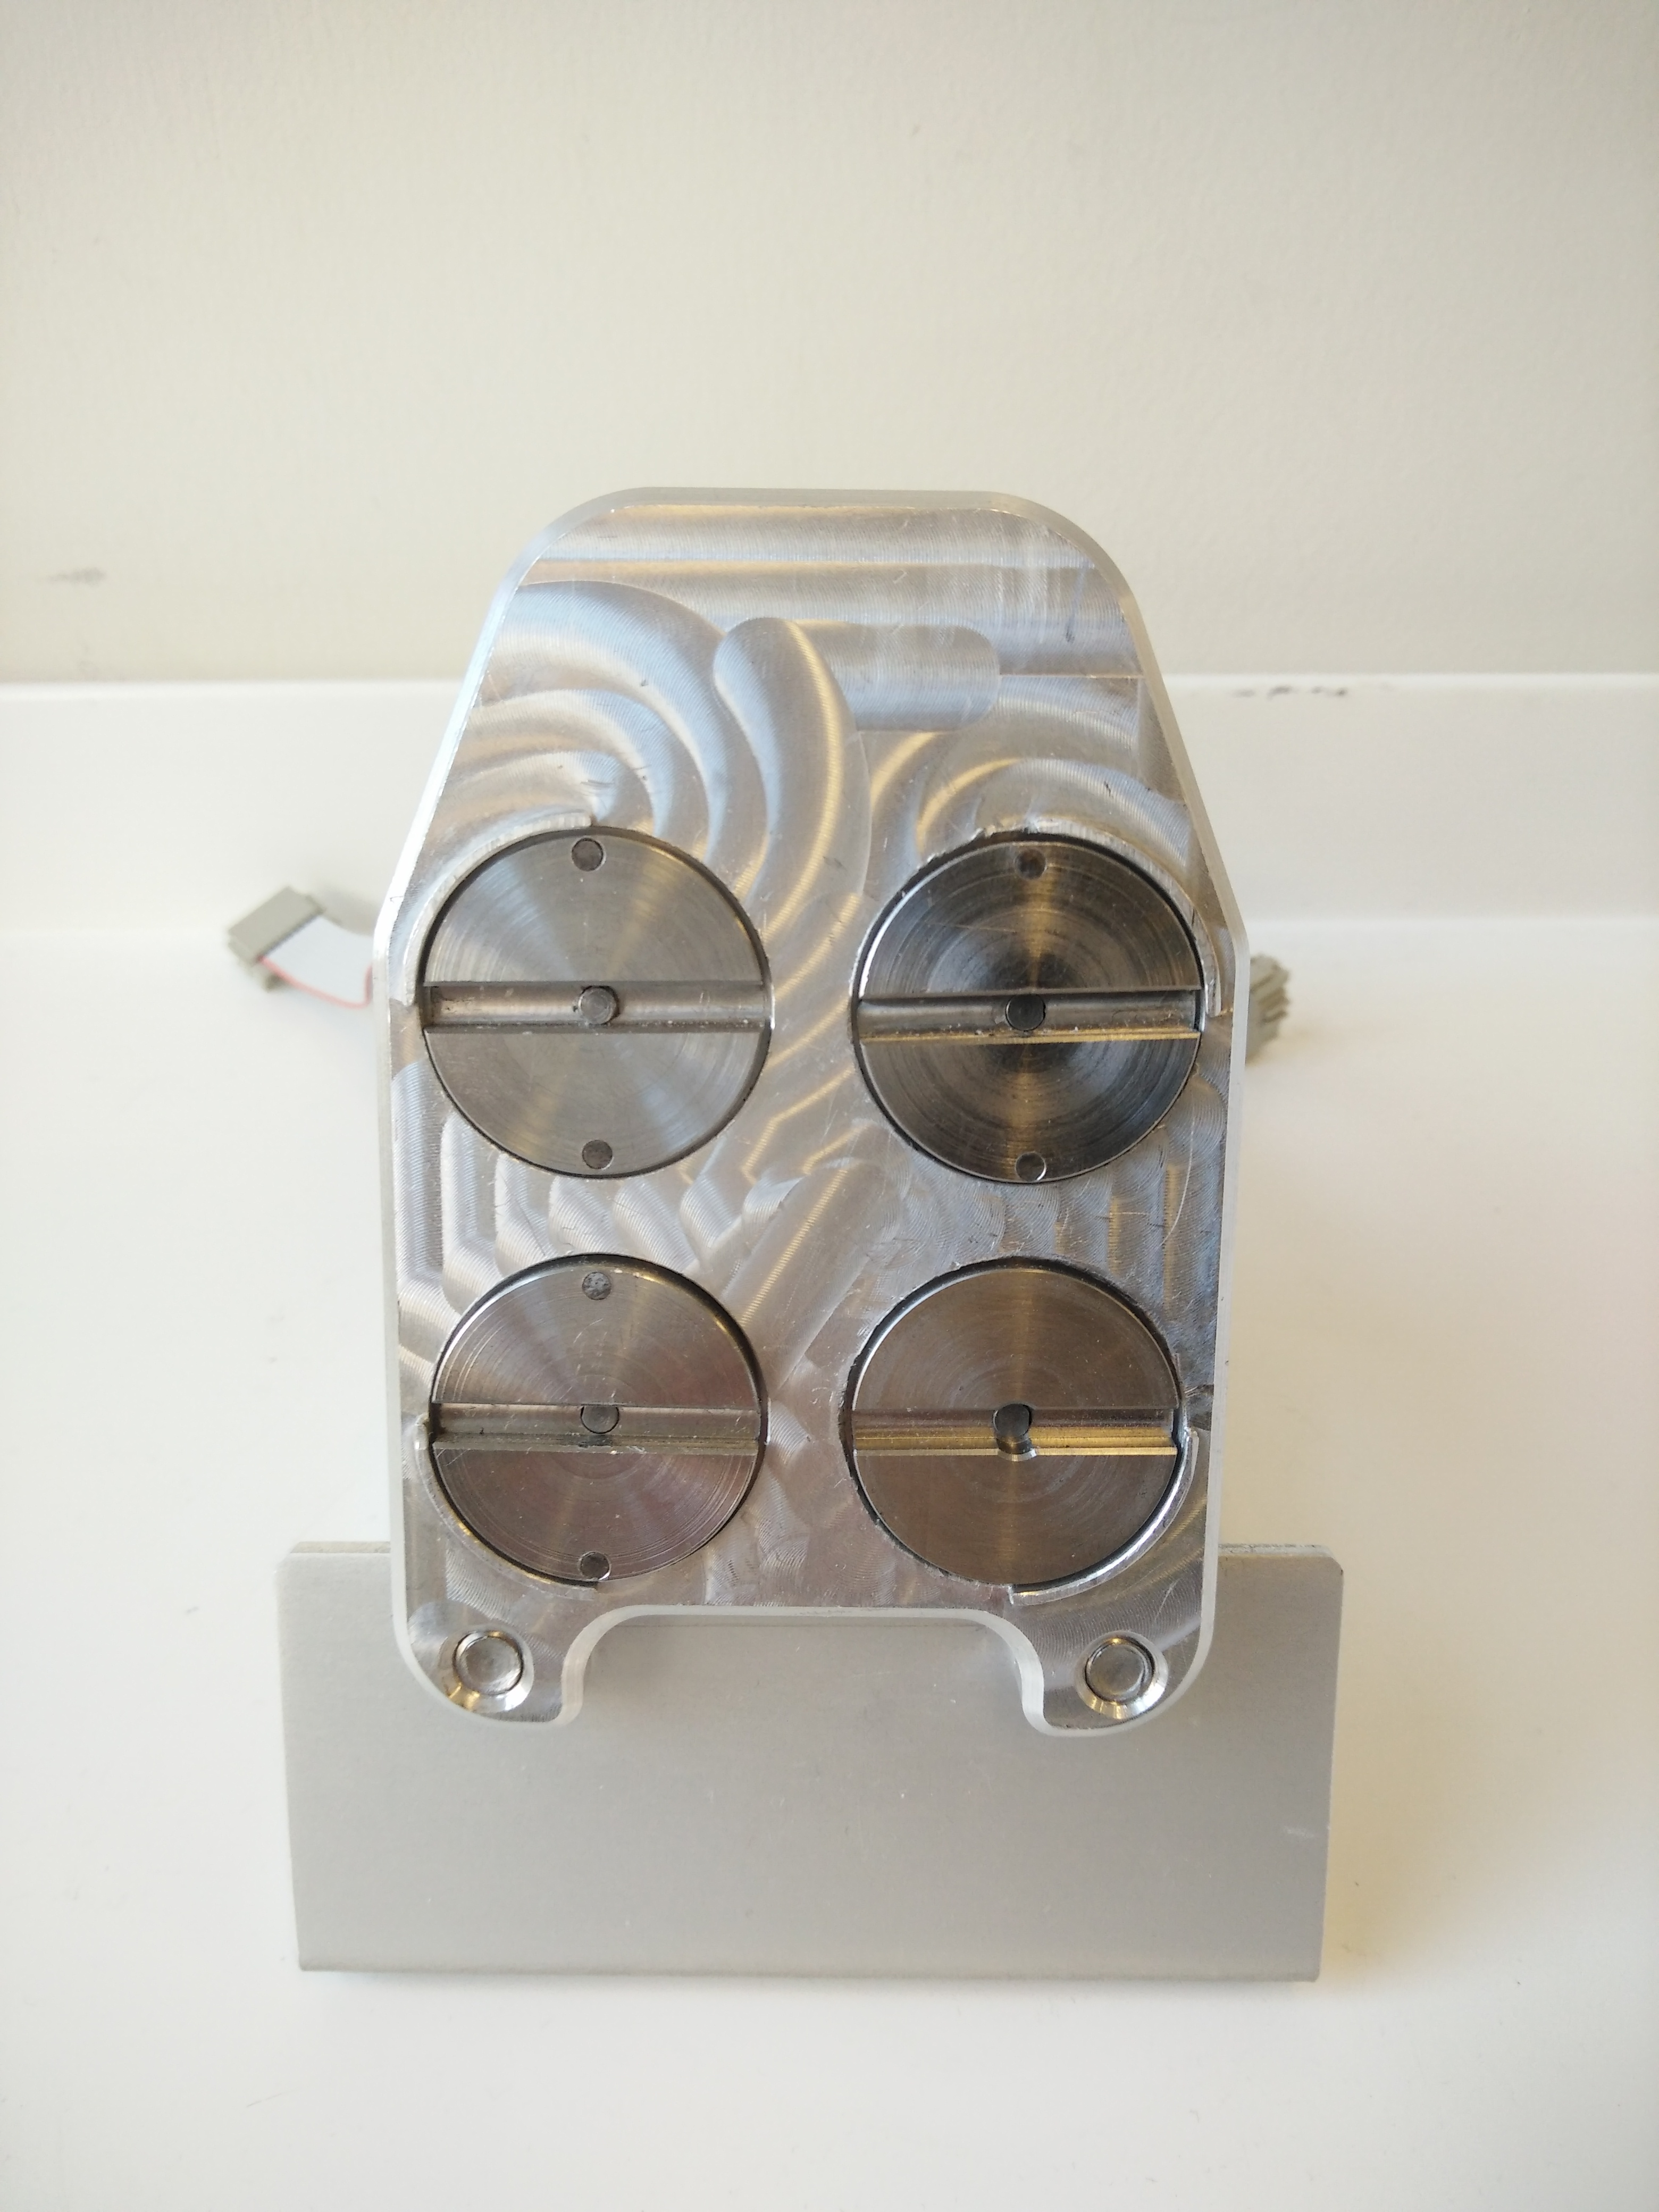
\includegraphics[width=\linewidth]{Test_setup1.jpg}
		\caption{EndoWrist holder. Front view}
		\label{fig:Mec_a}
	\end{subfigure}
	\hspace{\fill}
	\begin{subfigure}{0.45\textwidth}
		\centering
		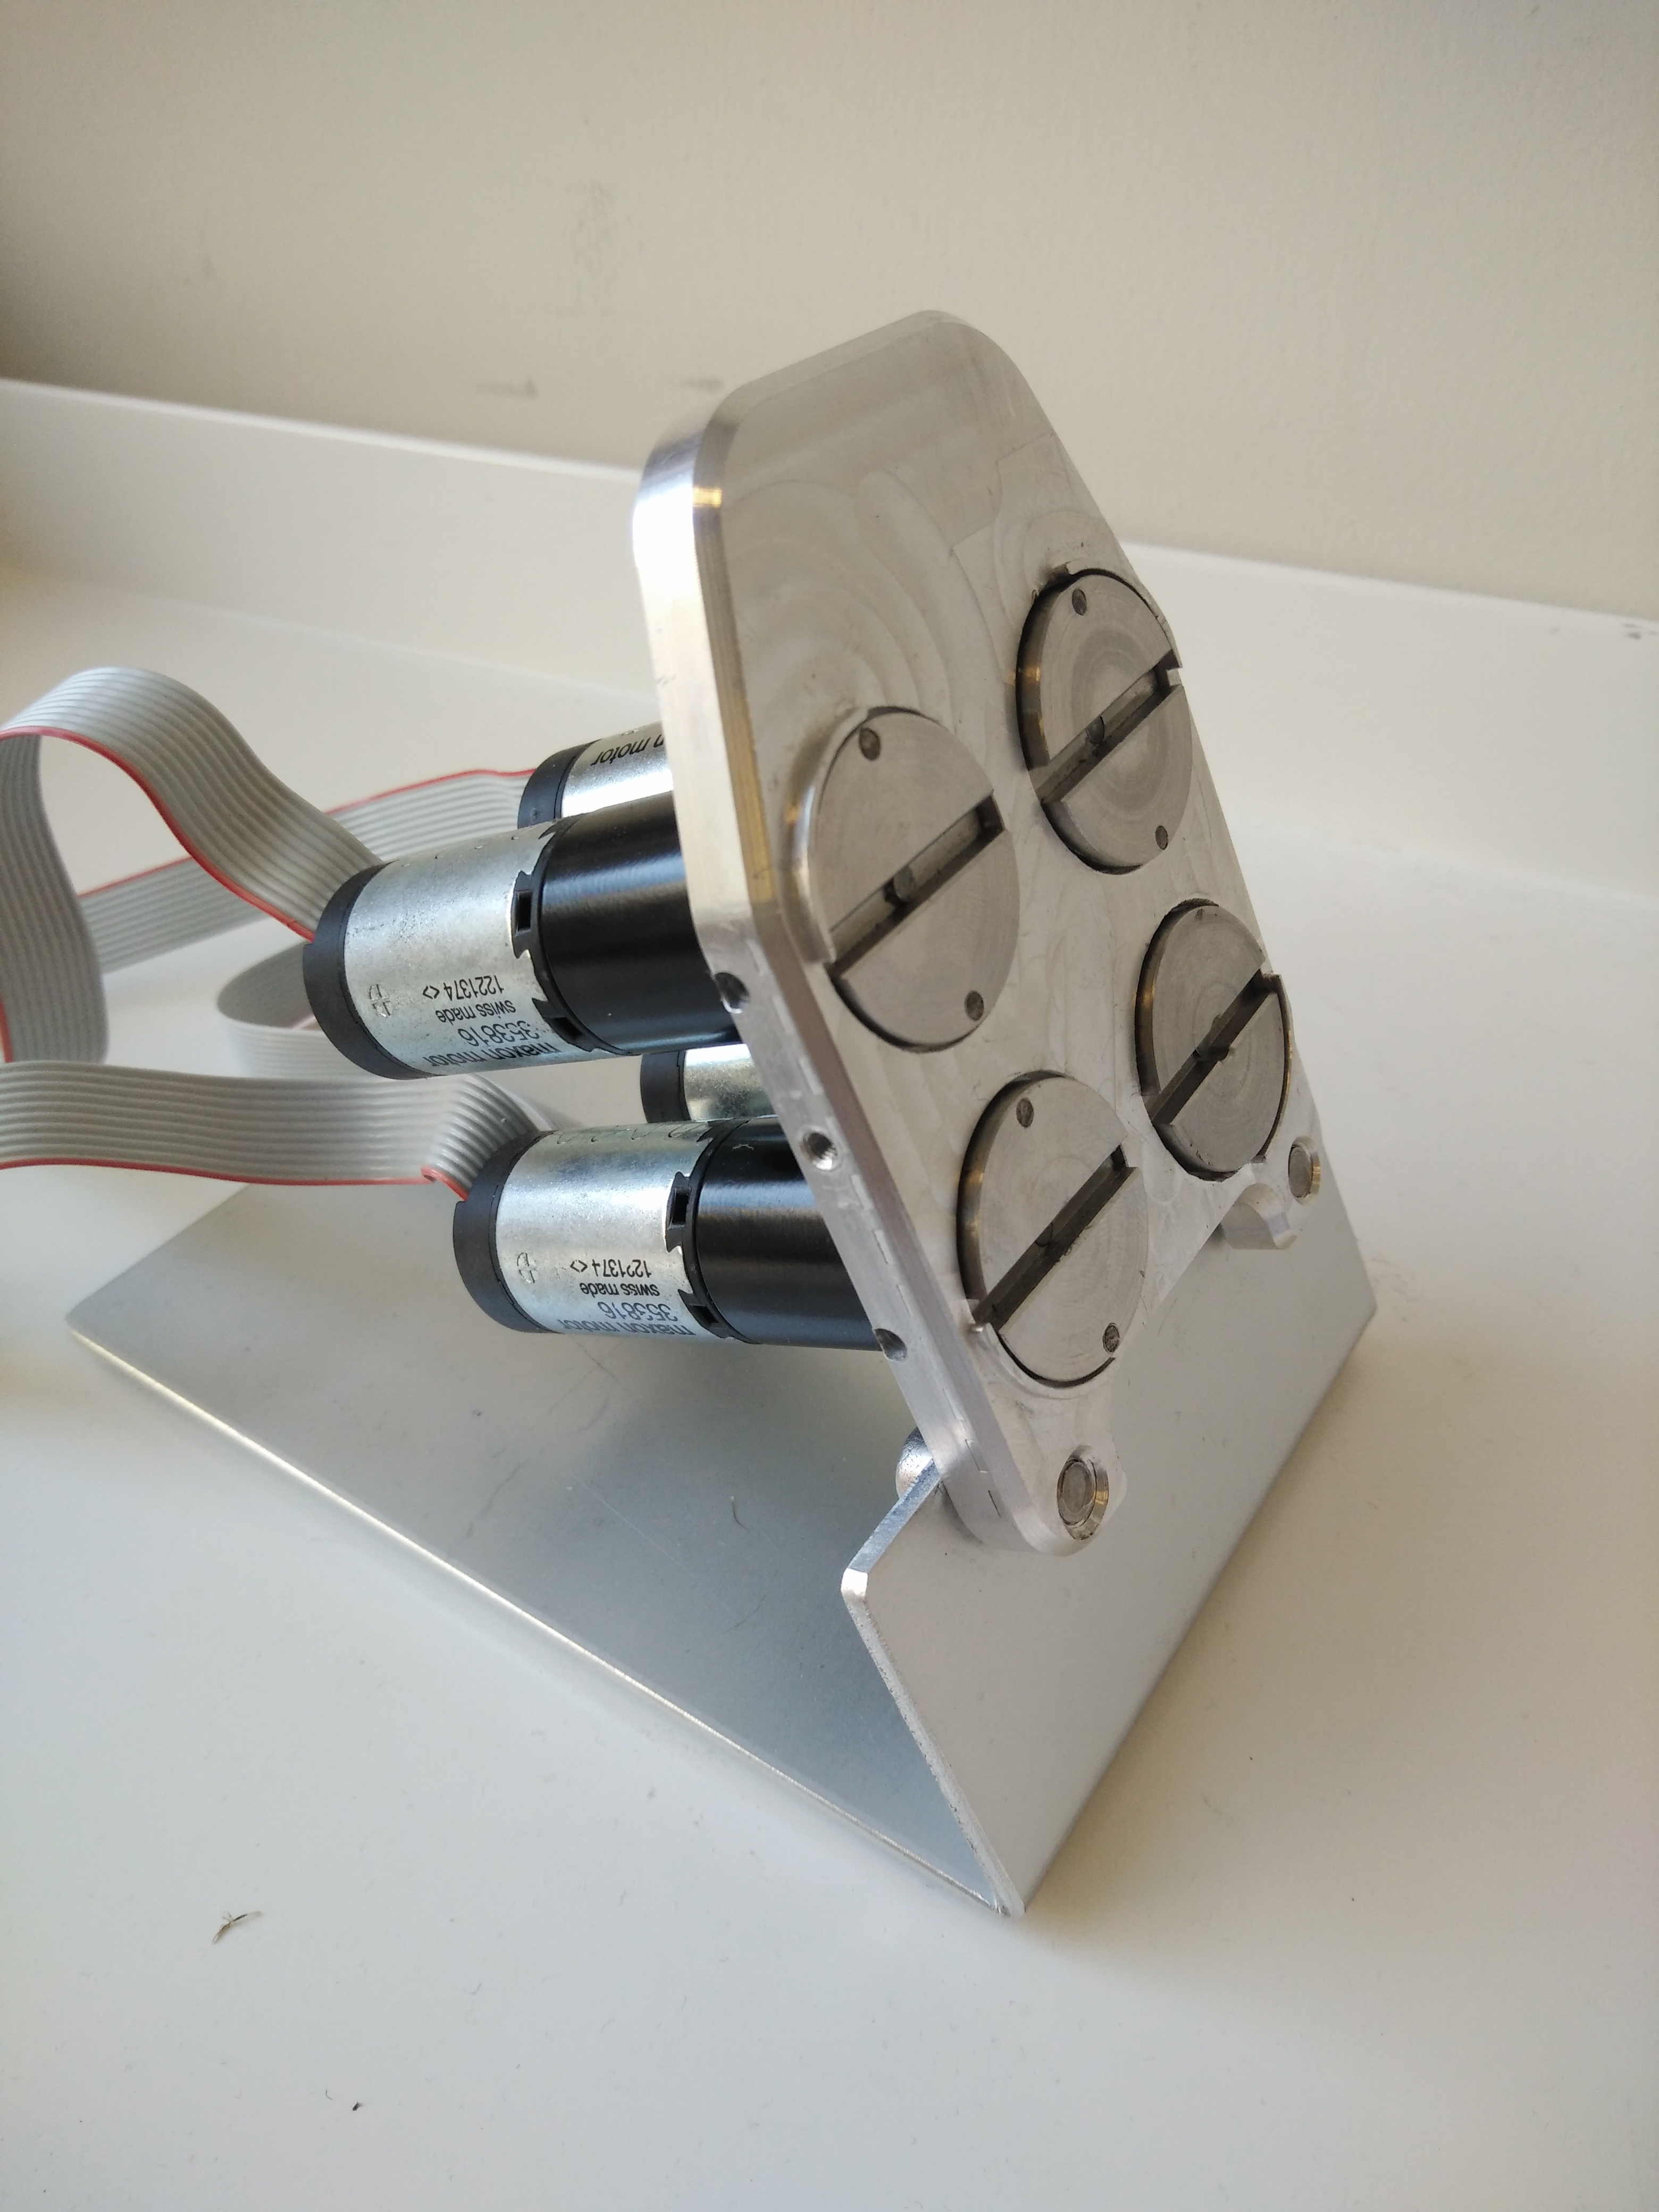
\includegraphics[width=\linewidth]{Test_setup2.jpg}
		\caption{EndoWrist holder with motors at the back. Side view}
		\label{fig:Mec_b}
	\end{subfigure}
	\end{minipage}

	\begin{minipage}[t]{0.9\textwidth}
	\vspace{20pt}
	\begin{subfigure}{0.45\textwidth}
		\vspace{0pt}
		\centering
		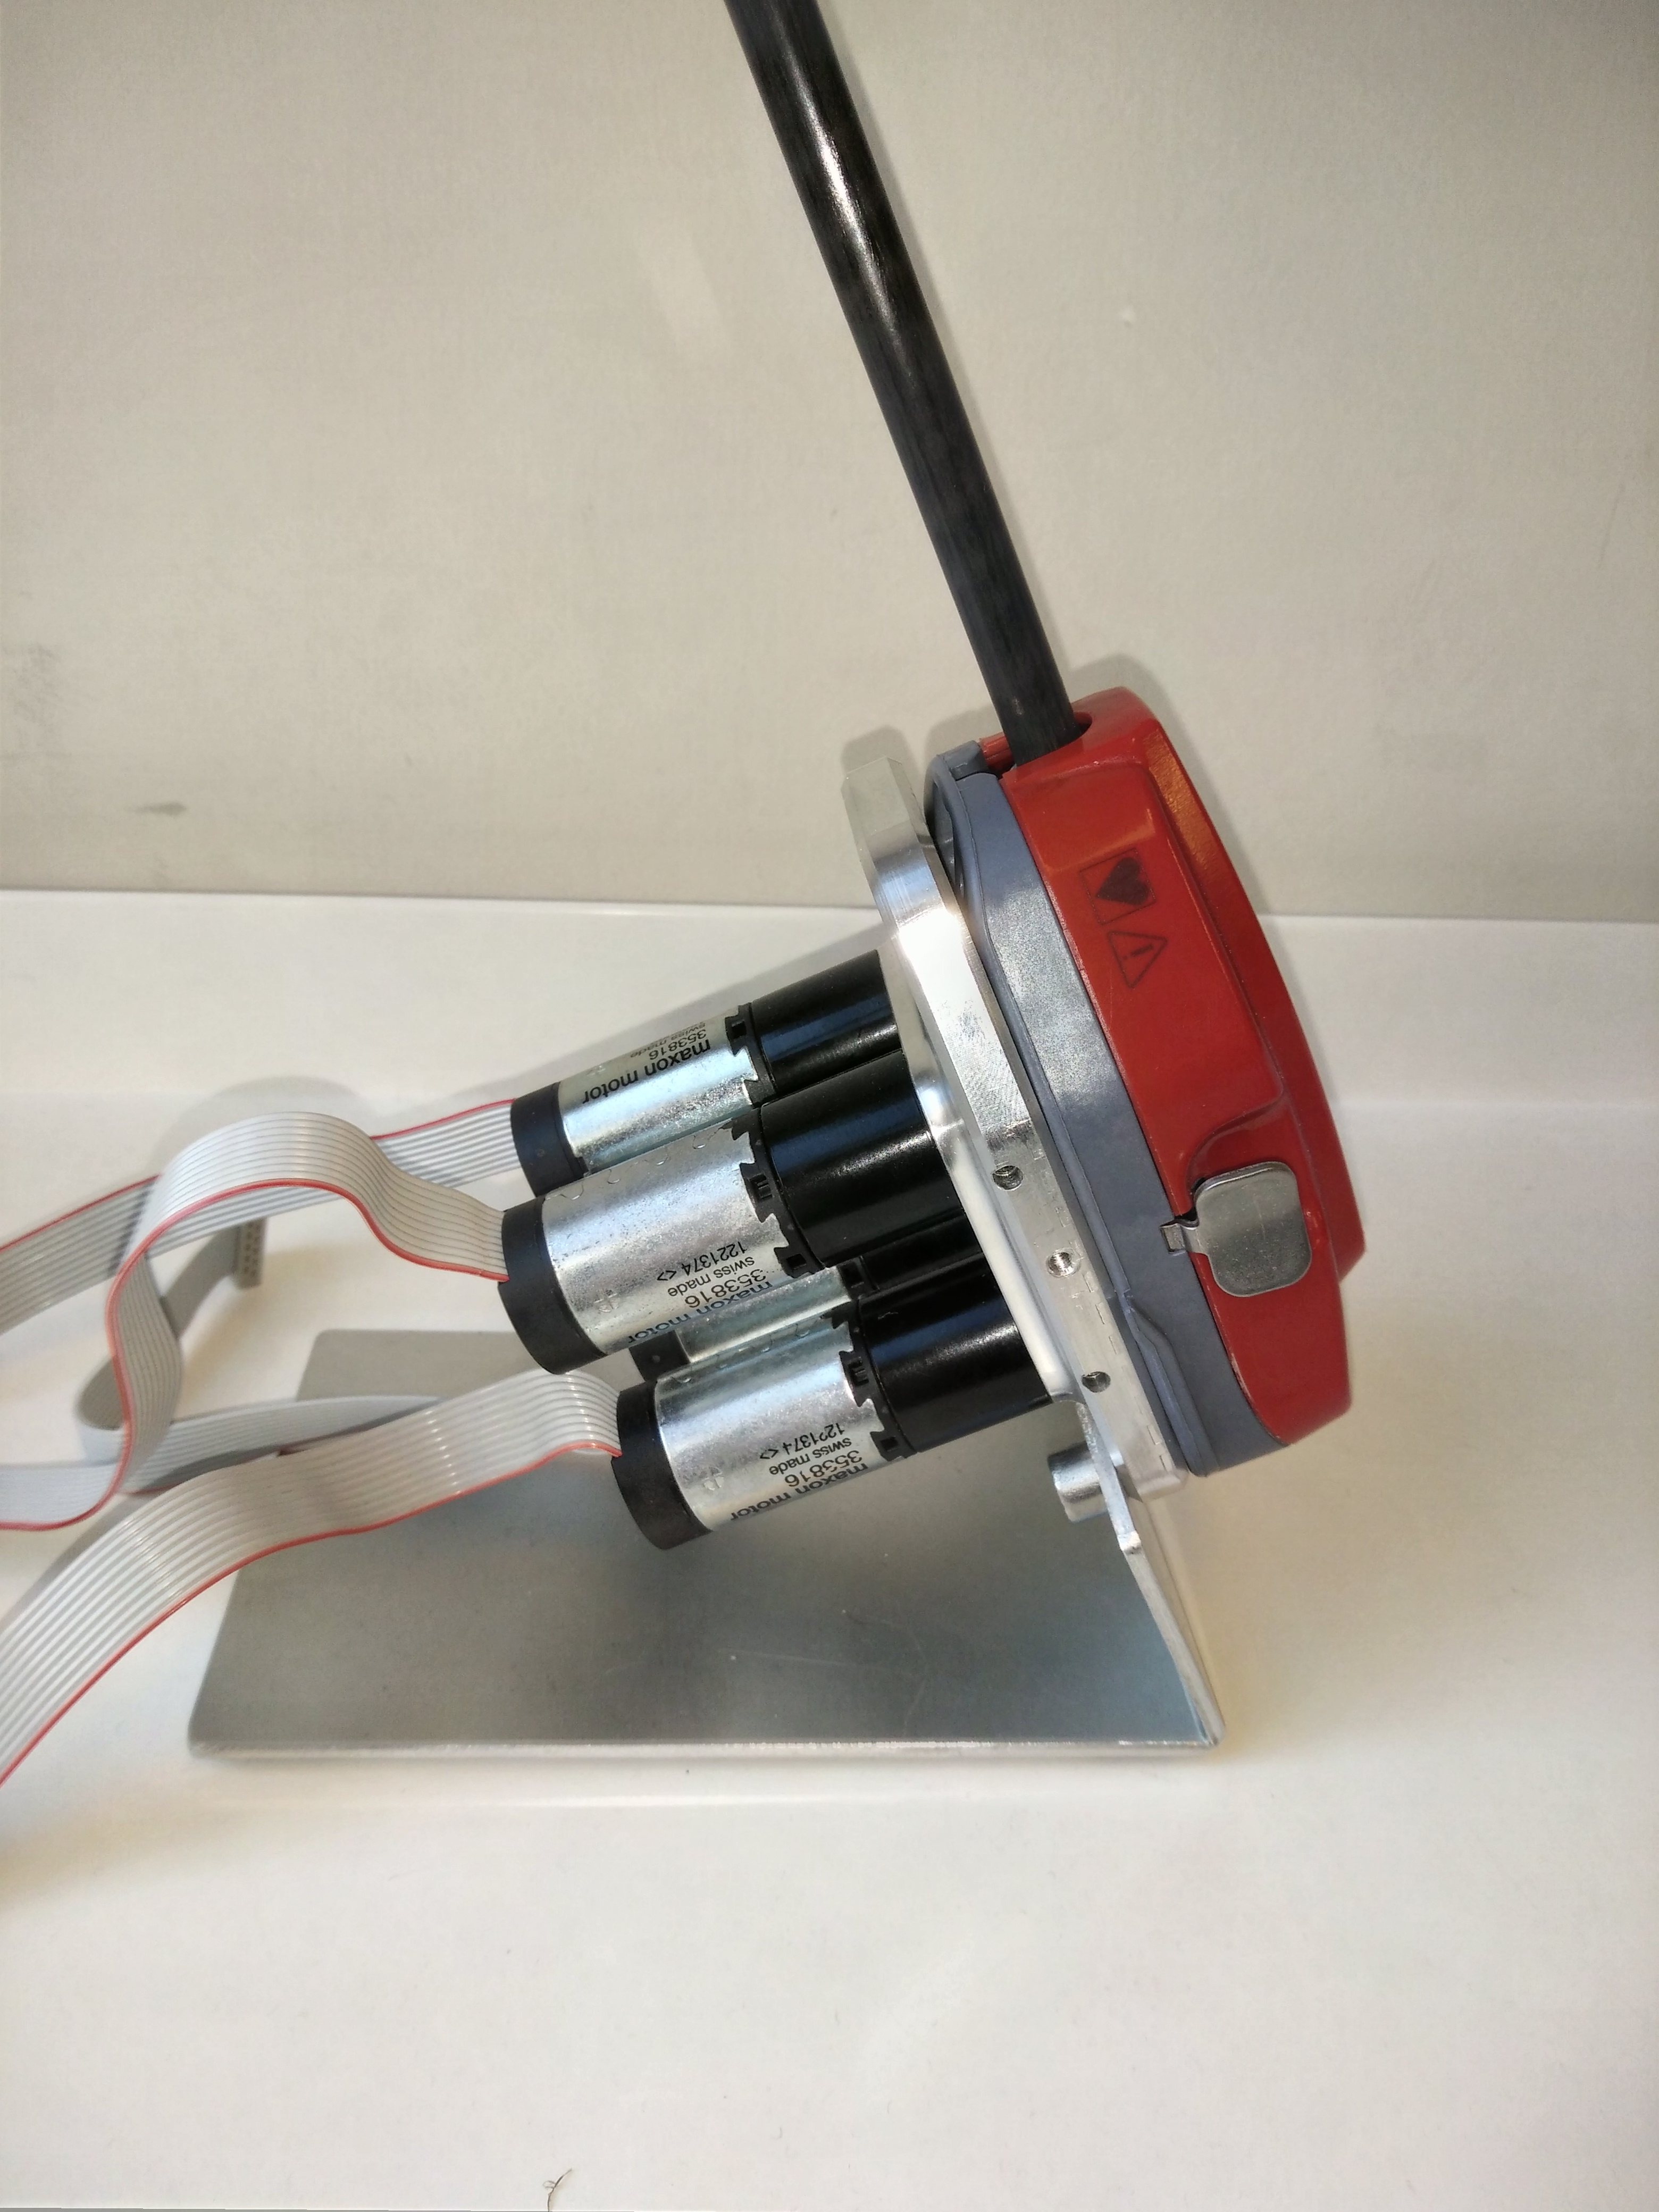
\includegraphics[width=\linewidth]{Test_setup3.jpg}
		\caption{EndoWrist holder with EndoWrist and motors. Side view}
		\label{fig:Mec_c}
	\end{subfigure}
	\hspace{\fill}
	\begin{subfigure}{0.45\textwidth}
		\centering
		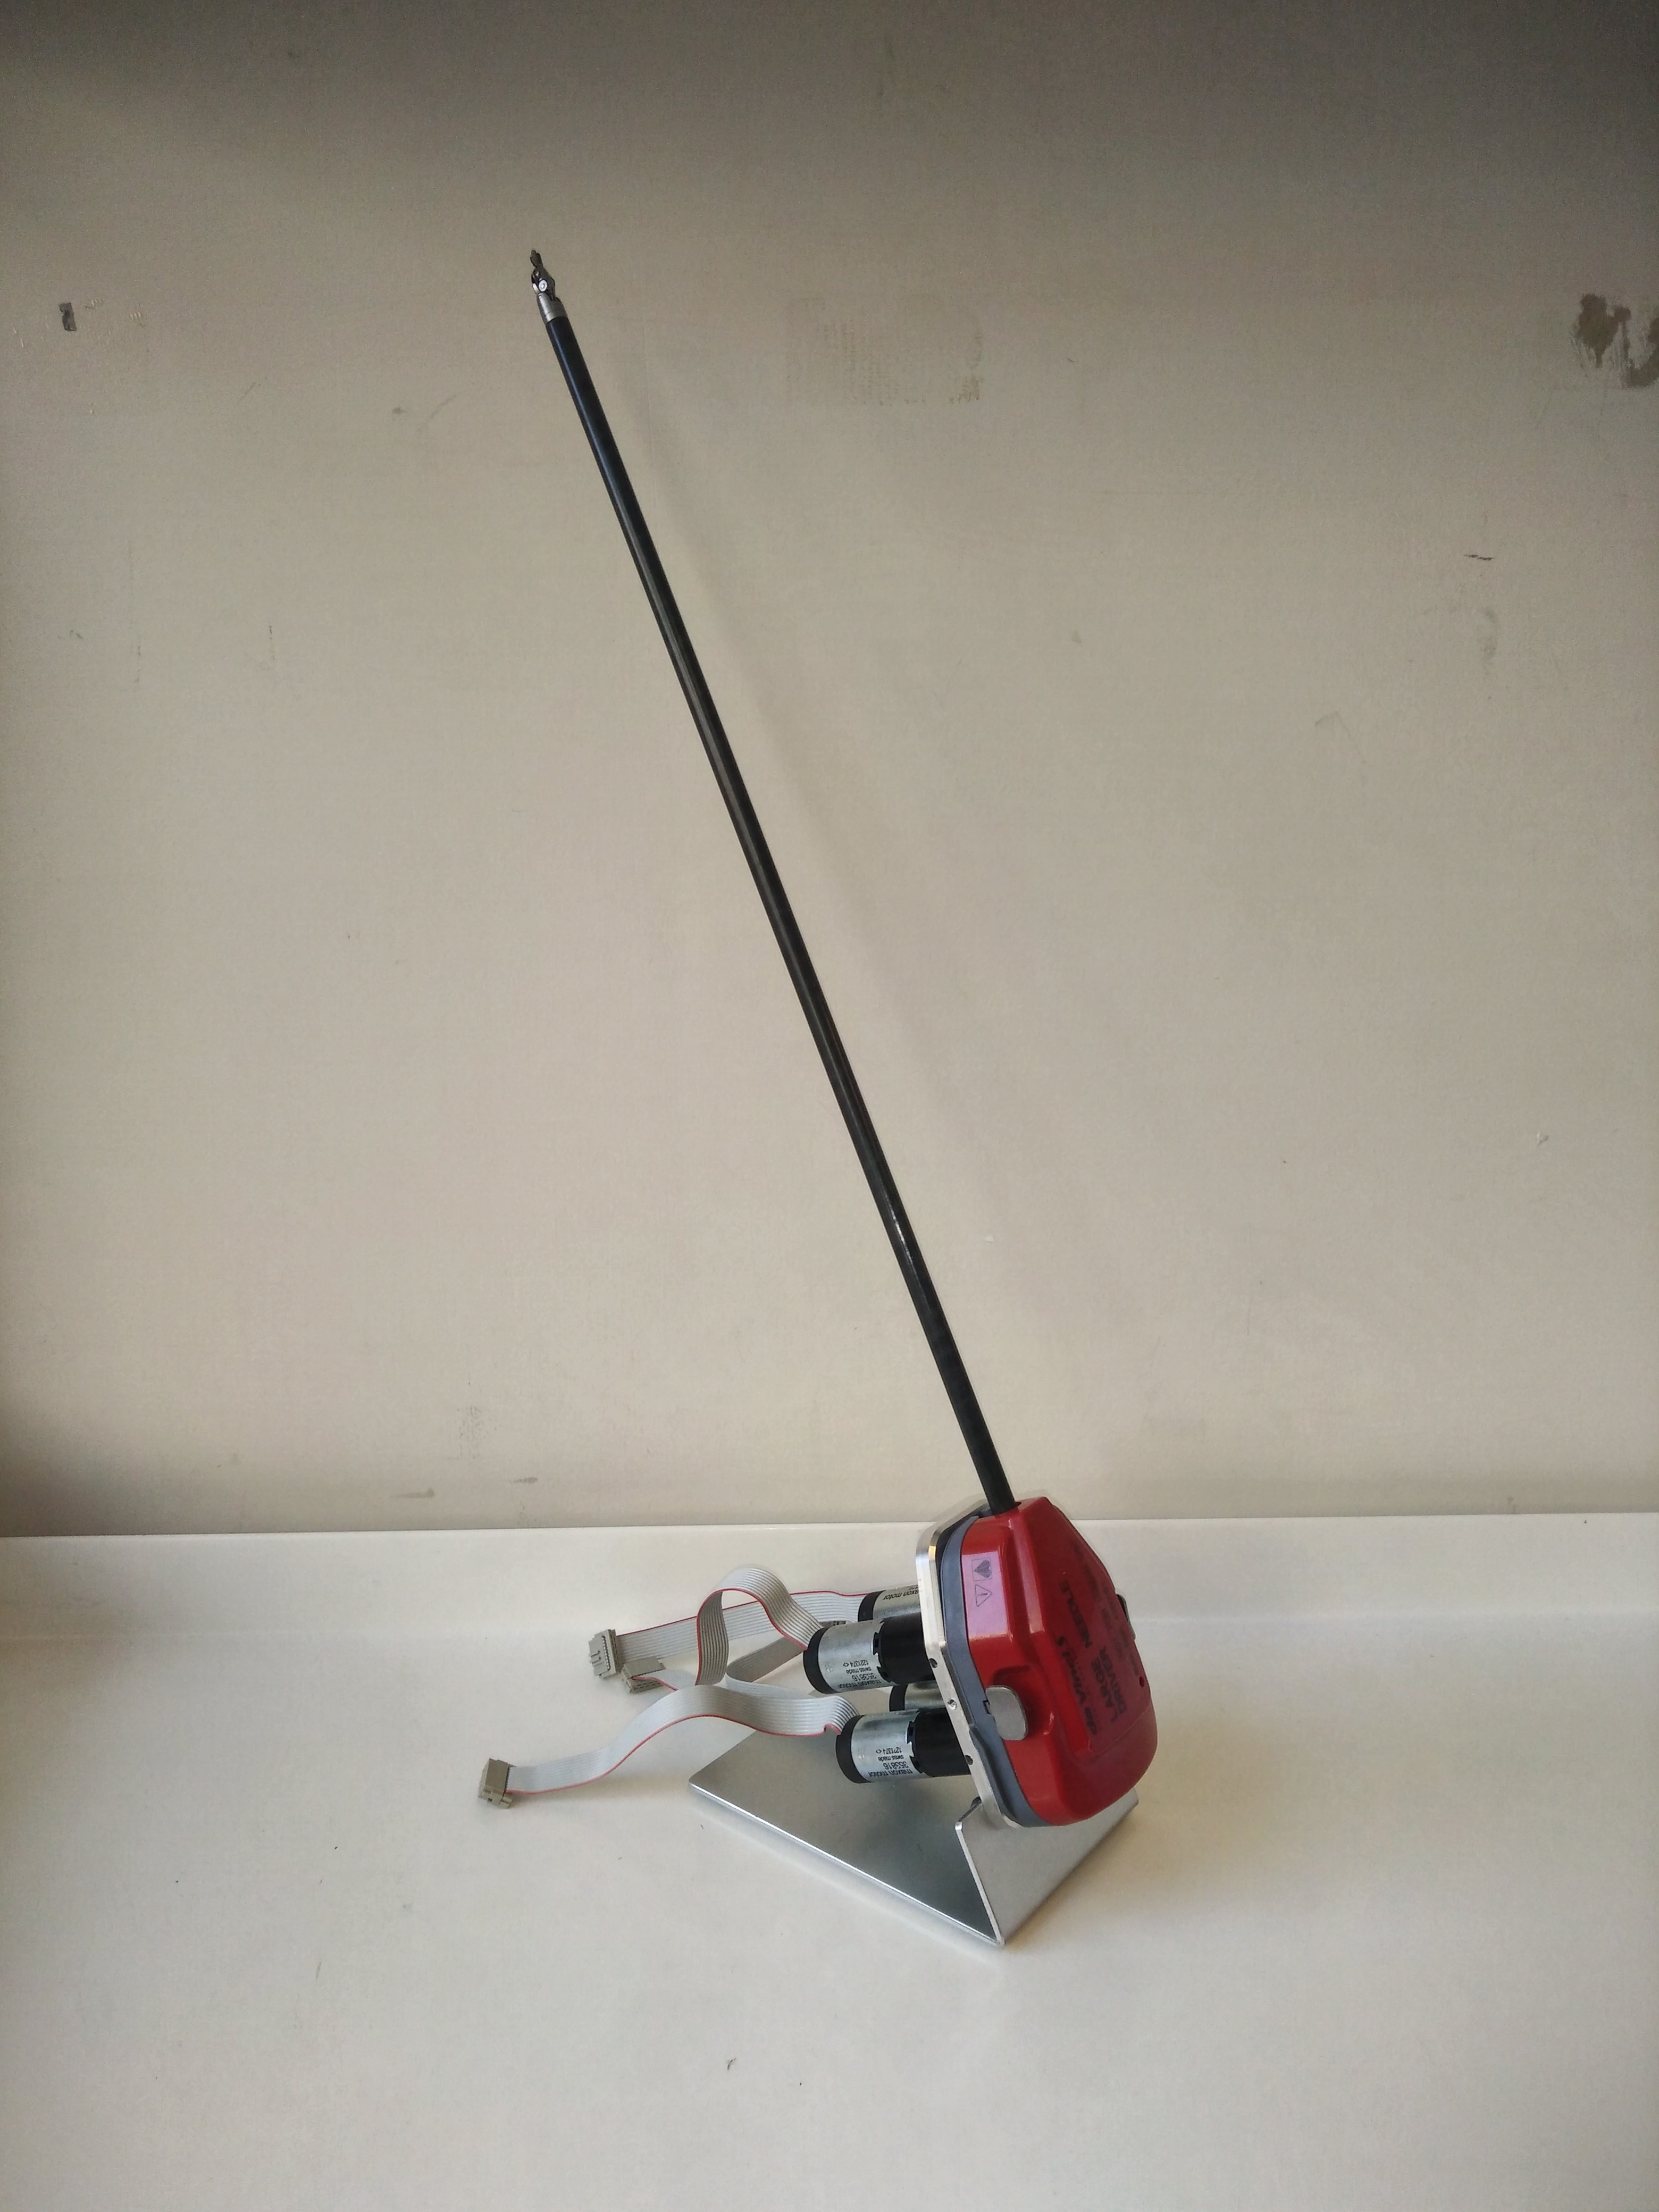
\includegraphics[width=\linewidth]{Test_setup4.jpg}
		\caption{Full view of the mechanical test setup}
		\label{fig:Mec_d}
	\end{subfigure}
	\end{minipage}

	\caption{Four pictures of the mechanical test setup available at Aalborg University, which include motors, EndoWrist and EndoWrist holder}
	\label{fig:Mec_abcd}
\end{figure}

This setup can manipulate the EndoWrist in the same manner as if the tool was connected to the da Vinci robot, i.e. it is able to actuate the rotational DOFs of the end-effector.